%%%%%%%%%%%%%%%%%%%%%%%%%%%%%%%%%% Chapter 6 %%%%%%%%%%%%%%%%%%%%%%%%%%%%%%%%%%
\chapter{Implementation \label{chapter:6}}
    This chapter will explain the code used in the thesis in detail. The code
    itself i given in >> REF GITHUB REPO <<. General information of the usage
    of packages are given in appendix >> REF APPENDIX << while the structure
    and workflow of the code is given here. We will first present a
    workflow-chart of the two main code-bases used, namely the Hartree-Fock
    implementation and the Variational Monte-Carlo implmentation.
    \begin{figure}[H]
        \centering
        \begin{subfigure}[b!]{0.49\textwidth}
            \centering
            \begin{tikzpicture}[
                    >={Latex[width=2mm,length=2mm]},
                        base/.style = {rectangle, rounded corners, draw=black,
                                    minimum width=4cm, minimum height=1cm, text
                                    centered, font=\sffamily},
                        activityStarts/.style = {base, fill=blue!30},
                        startstop/.style = {base, fill=red!30},
                        activityRuns/.style = {base, fill=green!30},
                        process/.style = {base, minimum width=2.5cm,
                        fill=orange!15, font=\ttfamily},
                    scale=0.8, 
                    node distance=1.5cm, 
                    every node/.style={fill=white, font=\sffamily},
                    align=center]
                \node (start)       [activityStarts]        {Bleh};
            \end{tikzpicture}
        \end{subfigure}
    \end{figure}

\section{Cartesian Basis}
    In \Arf{chapter:4} we mentioned the use of basis functions the different
    Many-Body methods. These can be pre-built using nifty intuition. One such
    observation is in the way harmonic oscillator functions station themselves
    on energy-levels(in the full-shell case). The following image\footnote{As
    the old idiom goes; "A picture is worth a thousand words"} describes this
    for the first few levels
        \begin{figure}[H]
            \centering
            \begin{subfigure}[b!]{0.49\textwidth}
                \centering
                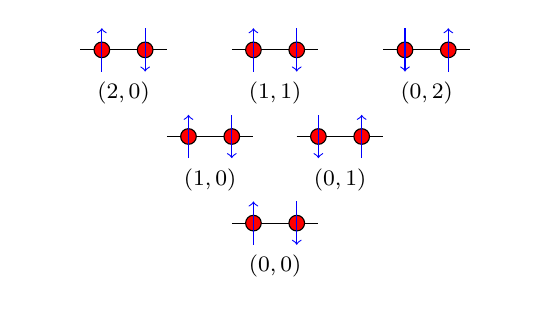
\begin{tikzpicture}[scale=0.55]
                    \draw (-1,0) -- (1,0);
                    \node at (-0.5,0) [draw,circle,fill=red,scale=0.6] {};
                    \node at (0.5,0) [draw,circle,fill=red,scale=0.6] {};
                    \draw[blue, ->] (-0.5,-0.5) -- (-0.5,0.5);
                    \draw[blue, <-] (0.5,-0.5) -- (0.5,0.5);
                    \node[text width=2.2cm, align=center] at (0,-1) {\footnotesize{$(0,0)$}};
                    \draw (-2.5,2) -- (-0.5,2);
                    \node at (-2.0,2) [draw,circle,fill=red,scale=0.6] {};
                    \node at (-1.0,2) [draw,circle,fill=red,scale=0.6] {};
                    \draw[blue, ->] (-2.0,1.5) -- (-2.0,2.5);
                    \draw[blue, <-] (-1.0,1.5) -- (-1.0,2.5);
                    \node[text width=2.2cm, align=center] at (-1.5,1) {\footnotesize{$(1,0)$}};
                    \draw (0.5,2) -- (2.5,2);
                    \node at (1.0,2) [draw,circle,fill=red,scale=0.6] {};
                    \node at (2.0,2) [draw,circle,fill=red,scale=0.6] {};
                    \draw[blue, <-] (1.0,1.5) -- (1.0,2.5);
                    \draw[blue, ->] (2.0,1.5) -- (2.0,2.5);
                    \node[text width=2.2cm, align=center] at (1.5,1) {\footnotesize{$(0,1)$}};
                    \draw (-4.5,4) -- (-2.5,4);
                    \node at (-4.0,4) [draw,circle,fill=red,scale=0.6] {};
                    \node at (-3.0,4) [draw,circle,fill=red,scale=0.6] {};
                    \draw[blue, ->] (-4.0,3.5) -- (-4.0,4.5);
                    \draw[blue, <-] (-3.0,3.5) -- (-3.0,4.5);
                    \node[text width=2.2cm, align=center] at (-3.5,3) {\footnotesize{$(2,0)$}};
                    \draw (-1,4) -- (1,4);
                    \node at (-0.5,4) [draw,circle,fill=red,scale=0.6] {};
                    \node at (0.5,4) [draw,circle,fill=red,scale=0.6] {};
                    \draw[blue, ->] (-0.5,3.5) -- (-0.5,4.5);
                    \draw[blue, <-] (0.5,3.5) -- (0.5,4.5);
                    \node[text width=2.2cm, align=center] at (0,3) {\footnotesize{$(1,1)$}};
                    \draw (4.5,4) -- (2.5,4);
                    \node at (4.0,4) [draw,circle,fill=red,scale=0.6] {};
                    \node at (3.0,4) [draw,circle,fill=red,scale=0.6] {};
                    \draw[blue, ->] (4.0,3.5) -- (4.0,4.5);
                    \draw[blue, <-] (3.0,3.5) -- (3.0,4.5);
                    \node[text width=2.2cm, align=center] at (3.5,3) {\footnotesize{$(0,2)$}};
                \end{tikzpicture}
                \caption{Two-dimensional case with $(n_x,n_y)$ notation.}
                \label{subfig:2Dspin}
            \end{subfigure}
            \begin{subfigure}[b!]{0.49\textwidth}
                \centering
                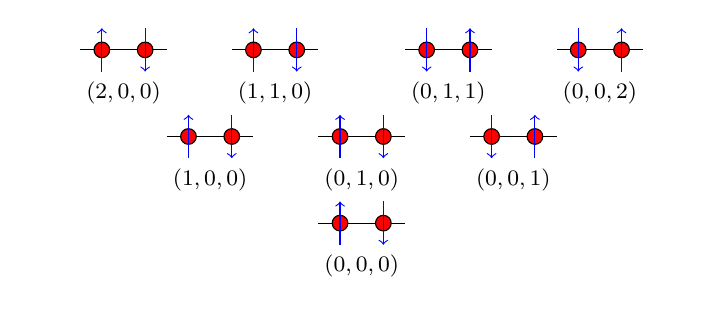
\begin{tikzpicture}[scale=0.55]
                    \draw (-1,0) -- (1,0);
                    \node at (-0.5,0) [draw,circle,fill=red,scale=0.6] {};
                    \node at (0.5,0) [draw,circle,fill=red,scale=0.6] {};
                    \draw[blue, ->] (-0.5,-0.5) -- (-0.5,0.5);
                    \draw[blue, <-] (0.5,-0.5) -- (0.5,0.5);
                    \node[text width=3.5cm, align=center] at (0,-1) {\footnotesize{$(0,0,0)$}};
                    \draw (-4.5,2) -- (-2.5,2);
                    \node at (-4.0,2) [draw,circle,fill=red,scale=0.6] {};
                    \node at (-3.0,2) [draw,circle,fill=red,scale=0.6] {};
                    \draw[blue, ->] (-4.0,1.5) -- (-4.0,2.5);
                    \draw[blue, <-] (-3.0,1.5) -- (-3.0,2.5);
                    \node[text width=2.2cm, align=center] at (-3.5,1) {\footnotesize{$(1,0,0)$}};
                    \draw (-1,2) -- (1,2);
                    \node at (-0.5,2) [draw,circle,fill=red,scale=0.6] {};
                    \node at (0.5,2) [draw,circle,fill=red,scale=0.6] {};
                    \draw[blue, ->] (-0.5,1.5) -- (-0.5,2.5);
                    \draw[blue, <-] (0.5,1.5) -- (0.5,2.5);
                    \node[text width=2.2cm, align=center] at (0,1) {\footnotesize{$(0,1,0)$}};
                    \draw (2.5,2) -- (4.5,2);
                    \node at (3.0,2) [draw,circle,fill=red,scale=0.6] {};
                    \node at (4.0,2) [draw,circle,fill=red,scale=0.6] {};
                    \draw[blue, <-] (3.0,1.5) -- (3.0,2.5);
                    \draw[blue, ->] (4.0,1.5) -- (4.0,2.5);
                    \node[text width=2.2cm, align=center] at (3.5,1) {\footnotesize{$(0,0,1)$}};
                    \draw (-6.5,4) -- (-4.5,4);
                    \node at (-6.0,4) [draw,circle,fill=red,scale=0.6] {};
                    \node at (-5.0,4) [draw,circle,fill=red,scale=0.6] {};
                    \draw[blue, ->] (-6.0,3.5) -- (-6.0,4.5);
                    \draw[blue, <-] (-5.0,3.5) -- (-5.0,4.5);
                    \node[text width=2.2cm, align=center] at (-5.5,3) {\footnotesize{$(2,0,0)$}};
                    \draw (-3.0,4) -- (-1.0,4);
                    \node at (-2.5,4) [draw,circle,fill=red,scale=0.6] {};
                    \node at (-1.5,4) [draw,circle,fill=red,scale=0.6] {};
                    \draw[blue, ->] (-2.5,3.5) -- (-2.5,4.5);
                    \draw[blue, <-] (-1.5,3.5) -- (-1.5,4.5);
                    \node[text width=2.2cm, align=center] at (-2.0,3) {\footnotesize{$(1,1,0)$}};
                    \draw (3.0,4) -- (1.0,4);
                    \node at (2.5,4) [draw,circle,fill=red,scale=0.6] {};
                    \node at (1.5,4) [draw,circle,fill=red,scale=0.6] {};
                    \draw[blue, ->] (2.5,3.5) -- (2.5,4.5);
                    \draw[blue, <-] (1.5,3.5) -- (1.5,4.5);
                    \node[text width=2.2cm, align=center] at (2.0,3) {\footnotesize{$(0,1,1)$}};
                    \draw (6.5,4) -- (4.5,4);
                    \node at (6.0,4) [draw,circle,fill=red,scale=0.6] {};
                    \node at (5.0,4) [draw,circle,fill=red,scale=0.6] {};
                    \draw[blue, ->] (6.0,3.5) -- (6.0,4.5);
                    \draw[blue, <-] (5.0,3.5) -- (5.0,4.5);
                    \node[text width=2.2cm, align=center] at (5.5,3) {\footnotesize{$(0,0,2)$}};
                \end{tikzpicture}
                \caption{Three-dimensional case with $(n_x,n_y,n_z)$ notation.}
                \label{subfig:3Dspin}
            \end{subfigure}
            \caption{Harmonic Oscillator Levels}
            \justify
        \end{figure}
    This specific arrangement of basis-functions is implemented in class
    \hltexttt{Cartesian} and is used in both the Hartree-Fock and VMC
    implementations. It essentially builds a matrix of states with the rows
    being the specific state and the columns containing the quantum numbers(in
    cartesian), the spin-value(as an integer), magic number and energy(in
    natural units proportional to the oscillator frequency). The essential form
    is
        \begin{equation}
            \begin{aligned}
                \begin{pmatrix}
                    n_x & n_y & s & m_s & E & M
                \end{pmatrix}
                \indent
                \begin{pmatrix}
                    n_x & n_y & n_z & s & m_s & E & M
                \end{pmatrix}
            \end{aligned}
        \end{equation}
    with the $n$'s being the principal numbers, $s$ the spin value $m_s$ the
    spin projection(up or down in our case), $E$ the energy and $M$ the magic
    number. The \hltexttt{Cartesian} class builds the states with alternating
    spin (the spacial parts are doubled with spin), but also has a function for
    restructuring by setting the states with spin down in acending order first
    and the same states with spin up after.

\section{Hartree-Fock}
    The Hartree-Fock method described in \Arf{sec:HFtheory} is implemented in
    >> REF GITHUB <<. Only the restricted case is implemented and is present as
    the class \hltexttt{HartreeFockSolver}. The matrix-elements(integrals) are
    implemented in \hltexttt{HermiteIntegrals} class. This class also uses an
    auto-generated header for the Hermite-coefficients, see
    \Arf{sec:auto_generation} below. The \hltexttt{HartreeFockSolver} is
    implemented in a general way such that an abstract class for the integral
    elements is all that is needed. The \hltexttt{HartreeFockSolver} can then
    be inherited and used.  An example of how to create a solver object with
    the Double-Well system called HFS with number of dimensions $D$, number of
    basis functions $L$ and number of particles $N$.
        \begin{lstlisting}[language=C++, style=ccstyle]
            DoubleWell* HFS = new DoubleWell(D, L, N);
            string message = HFS->initializeParameters(...);
        \end{lstlisting}
    With the $\dots$ meaning one initializes it with in however manner the
    function was made. The initialization function must also return a message
    determined by the success of the initialization. If it succeeds it return
    an empty message while if not it returns a pre-defined message. \\ 
    Here is a simple example code-snippet which initializes and runs the
    Hartree-Fock algorithm
        \begin{lstlisting}[language=C++, style=ccstyle]
            DoubleWell* HFS = new DoubleWell(D, L, N);

            string message = HFS->initializeParameters(...);
            if (message.compare("")) {
                if (myRank == 0) {
                    std::cout << message << std::endl;
                } // end if
                delete HFS;
                finalize();
            } // end if

            double E = HFS->iterate(M, 1e-8, true);
        \end{lstlisting}
    The \hltexttt{iterate} function takes in $M$ as the maximum number of
    iterations, the convergence tolerance (when to break the iteration) and a
    boolean for showing progress or not. It calculates the integral-elements
    and runs the Hartree-Fock algorithm and returns the estimation of the
    ground-state energy. >> REF (NOT REALLY) EXPLAIN INPUTS <<

\subsection{Parallelization of Two-Body Matrix}
    The most time-consuming part of the Hartree-Fock procedure is the
    calculation of the two-body matrix-elements giving the interaction terms.
    This is parallelized in the \hltexttt{assemble} function in
    \hltexttt{HartreeFockSolver}. The basic premise is to represent the $N^4$
    elements $\Braket{pq|r^{-1}|rs}$ as a one-dimensional array with the mapping
        \begin{equation}
            (p,q,r,s) \rarr p + N(q + N(r + Ns))
        \end{equation}
    that is the element $(p,q,r,s)$ is stored in position $(p + N(q + N(r +
    Ns))$ in the one-dimensional array. The symmetry $(p,q,r,s)=(q,p,r,s)$
    reduces the number of elements down to $N(N+1)/2$. A $N(N+1)/2\times 2$
    matrix of indices is then created with
        \begin{algorithm}[H]
            \caption{Parallelization Index Mapping}\label{alg:paraindiexmap}
            \begin{algorithmic}[H]
                \State Initialize matrix pqMap with $\frac{N}{2}(N+1)$ rows and
                $2$ columns.
                \State j = 0
                \For{p=0 : N-1}
                    \For{q=p : N-1}
                        \State pqMap[j,0] = p
                        \State pqMap[j,1] = q
                        \State j = j + 1
                    \EndFor
                \EndFor
            \end{algorithmic}
        \end{algorithm}
    The rows are then distributed evenly among $P$ processes according to
        \begin{equation}
            \text{rows} = \left\{\begin{aligned}
                \left\lceil\frac{\frac{N}{2}(N+1)}{P}\right\rceil &\indent&
                &\text{rank} < \left(\frac{N}{2}(N+1)\mod P\right) \\
                \left\lfloor\frac{\frac{N}{2}(N+1)}{P}\right\rfloor
                &\indent& &\text{else}
                \end{aligned}\right.
        \end{equation}
    The problem now however is that processes of higher and higher ranks my end
    up with calculating more since larger indices involve computationally more
    heavy functions to be evaluated. We can account for this by weighting the
    number of rows each process gets by the sum of the indices. The algorithm
    is as follows
        \begin{algorithm}[H]
            \caption{Even Weighting}\label{alg:parasumweight}
            \begin{algorithmic}[H]
                \State Make array $S$ of size $P$ with each element being the
                sum of the $(p,q)$ elements for the specific process.
                \State Make an array sizes of size $P$ with the number of
                elements for each process.
                \State Make an array displ of size $P$ with the displacement
                (index).
                \State $O =$ Mean of $S$.
                \For{$i=0$ to $P-2$}
                    \For{$j=$displ$[i]$ to displ$[i]+$sizes$[i+1]$} 
                    \Comment{Iterate over elements in right adjacent process.}
                        \State $L = S[i] + $sum(pqMap.row($j$))
                        \If{$L < O$}
                            \State sizes$[i] =$ sizes$[i] + 1$
                            \State sizes[$i+1$] = sizes[$i+1$]$ - 1$;
                            \State displ[$i+1$] = displ[$i+1$]$ + 1$;
                        \ElsIf{$L$ equals $O-1$ or $L$ equals $O+1$ or $L>O$}
                            \State Break inner-most loop.
                        \EndIf
                    \EndFor
                    \State Set elements of $S$.
                \EndFor
            \end{algorithmic}
        \end{algorithm}
    Each process has access to the \hltexttt{pqMap} array such that the each
    process calculates its own chunk according to the size set and the
    \hltexttt{displ} tells the start-index. Each process then calculates the
    two-body elements according to
        \begin{algorithm}[H]
            \caption{Two-Body Calculation}\label{alg:paratwobody}
            \begin{algorithmic}[H]
                \State Initialize $A$ for containing $(p,q,r,s)$ elements.
                \State Initialize $B$ for containing $(p,q,s,r)$ elements.
                \State $i_{\text{start}} =$ displ[rank]
                \State $i_{\text{end}} =$ displ[rank] $+$ sizes[rank]
                \State $k=0$
                \For{$l=i_{\text{start}}$ to $i_{\text{end}}-1$}
                    \For{$r=0$ to $N-1$}
                        \For{$s=r$ to $N-1$}
                            \State $p=$pqMap$[l,0]$
                            \State $q=$pqMap$[l,1]$
                            \State $A[l]=\Braket{pq|\frac{1}{r_{12}}|rs}$
                            \State $B[l]=\Braket{pq|\frac{1}{r_{12}}|sr}$
                        \EndFor
                    \EndFor
                \EndFor
            \end{algorithmic}
        \end{algorithm}
    Each $A$ and $B$ is then sent to root process and concatenated to a large
    one-dimensional array and the actual two-body matrix of size $N^4$ is
    assembled and antisymmetrized. The Hartree-Fock algorithm is then run only
    on one process.
    
    >> make structure (image??) of HartreeFock::All structure)

\section{Variational Monte Carlo}
    The Variational Monte-Carlo implementation is mainly in three classes,
    namely \hltexttt{VMC}, \hltexttt{BruteForce} and
    \hltexttt{ImportanceSampling}. The structure is set such that both
    \hltexttt{BruteForce} and \hltexttt{ImportanceSampling} inherit
    \hltexttt{VMC}. This structure essentially gives room for splitting
    specific part of the Brute-Force algorithm from the Metropolis-Hastings
    algorithm, but still using the same code for minimization. We will explain
    the minimization parts in the next section. \\ 
    The main input which \hltexttt{VMC} needs is a wavefunction. An abstract
    class-template is implemented and can be generated using a python script,
    also given in the same GitHub repository >>REF GITHUB <<. The template is
    built in such a way that one only needs to fill in specific analytic
    expressions for the gradient, Laplacian and gradient for the variational
    parameters. The latter part is optional. \\ 
    The wavefunction itself is built using the \hltexttt{Slater} or
    \hltexttt{SlaterJastrow} class. However, in order to use the
    \hltexttt{SlaterJastrow} one has to specify which Jastrow function to use
    at compile time. A simple example illustrates this better
        \begin{lstlisting}[language=C++, style=ccstyle]
            SlaterJastrow* wf = new SlaterJastrow(dim, numParticles, parameters);
            wf->initializeParameters(omega);
            wf->initializeMatrices();

            ImportanceSampling<SlaterJastrow>* vmc = new
                    ImportanceSampling<SlaterJastrow>(stepmc, parameters,
                    maxIterations, rank, numProcs);

            double E = vmc->sampler();

            delete vmc;
            delete wf;
        \end{lstlisting}
    The first chunk initializes the SlaterJastrow class with the pre-specified
    system which needs to be given at compile time as a flag i.e
    WAVEFUNCTION=HarmonicOscillator. The second part sets the sampling to use
    Metropolis-Hastings algortithm. The parameters variable must be an
    \hltexttt{Eigen} >>REF EIGEN<< vector or array and contains the variational
    parameters present. The representation of each element in this vector(or
    array) is specific to each system. For a more detailed explanation see >>
    REF GITHUB <<. \\
    This is just an example of how to build a simple run, however we have also
    built a run file which uses YAML >> REF THIS <<. The basic template is as
    follows
        \begin{lstlisting}[language=yaml]
            omega: 1.0
            numparticles: 6
            maxitermc: 100000
            stepmc: 0.01
            parameters: [0.99, 0.47] #optional
            numparameters: 2
            jastrow: true #optional
            importance: true #optional
        \end{lstlisting}
    This is a template used for the \hltexttt{HarmonicOscillator} with the
    Pad\'e-function as Jastrow factor. If the NQS-function is used an
    additional parameter 'numhiddenbias' giving the number of hidden biases
    used, is needed. Again, for more detail see >> REF GITHUB << \\ 
    This form of input makes it fairly simple to actually run the code for
    different systems with ease. One needs to compile with the specific flag
    for the system(wavefunction and Jastrow) and then supply an YAML input file
    at runtime.

\subsection{Slater Optimizations}
    In the Metropolis sampling we need access to the ratio of two determinants,
    namely the Slater wavefunction at the current state and the one at previous
    state. These are quite expensive to calculate\footnote{Actual complexity of
    a determinant is $n\times n$, with $n$ being the size of the Slater
    matrix.}. This can be overcome by using the fact that moving only
    \txtit{one} particle at each iteration also constitutes to a
    state-transition. Following \cite{vmc} and given row $i$ as the index for
    the row that is changed, the following expressions are valid
        \begin{equation}
            \begin{aligned}
                \frac{\Psi}{\Psi'} &= \sum_j \psi_{ij} \psi_{ji}'^{-1} \\
                \frac{\nabla_i \Psi}{\Psi} &= \sum_j \psi_{ij} \nabla_i
                \psi_{ji}^{-1} \\
                \frac{\nabla^2_i \Psi}{\Psi} &= \sum_j \psi_{ij} \nabla^2_i
                \psi_{ji}^{-1} \\
            \end{aligned}
        \end{equation}
    with $\Psi'$ being the wavefunction at previous state. One might ask now,
    but isn't this just worse? We have gone from needing two determinants to
    needing two inverses!? Fret not, the Sherman-Morrison\cite{shermorInv}
    formula for updating an inverse matrix if only one row has changed in the
    original matrix comes to the rescue. The elements of the inverse can by
    this be expressed as(with $i$ being the row that changed)
        \begin{equation}
            \psi^{-1}_{kj} = \left\{\begin{aligned}
                \psi'^{-1}_{kj} - \frac{\Psi}{\Psi'}\psi'^{-1}_{ki}
                \suml{l=1}{N}\psi_{il}\psi'^{-1}_{lj}, \indent j \neq i\\
                \frac{\Psi}{\Psi'}\psi'^{-1}_{ki}\psi'^{-1}_{ki}
                \suml{l=1}{N}\psi'_{il}\psi'^{-1}_{lj}, \indent j = i
            \end{aligned}\right.
        \end{equation}
    This means that the inverses and the determinant ratios can be calculated
    fully once before the sampling and then updated using the above formulas.
    This procedure is implemented in the \hltexttt{Slater} class.

\subsection{Jastrow Optimizations}
    The Jastrow factors presented in \Arf{susec:TWFJastrow,
    sususec:TWFPadeJastrow, sususec:NQSJastrow} also give rise to optimizations
    in the case of moving only one particle at a time. In particular, the
    Pade\'e function and the simple exponential can both be represented by a
    matrix of size $N\times D$ as
        \begin{equation}
            \blds{J} = 
                \begin{pmatrix}
                    \blds{J}(\blds{r}_1) \dots \blds{J}(\blds{r}_N)
                \end{pmatrix}
        \end{equation}
    Moving one particle at a time means only one column in $\blds{J}$ is
    changed meaning only that column needs to be updated. Additionally, the
    $\blds{J}$ matrix doesn't actually need to be present in the code since we
    are only interested in ratios $J/J'$. If only one index $i$ changes we have
        \begin{align}
            \frac{J}{J'} &= \exp(\sumll{i<j} \left(f_{ij} - f'_{ij}\right))
            \nonumber \\
            &= \exp(\sumll{i\neq j} f_{ij})
        \end{align}
    Notice that $i$ is fixed in the last step. \\
    The gradient of $J$ can be represented as a $N\times N\times D$ matrix
        \begin{equation}
            \nabla \blds{J} = 
                \begin{pmatrix}
                    0 & \nabla \blds{J}(\blds{r}_{1,2}) & \dots & \nabla
                    \blds{J}(\blds{r}_{1,N-1}) \\
                    \nabla \blds{J}(\blds{r}_{2,1}) & 0 & \dots & \nabla
                    \blds{J}(\blds{r}_{2,N-1} \\
                    \vdots & \vdots & \ddots & \vdots \\
                    \nabla \blds{J}(\blds{r}_{N,1}) & \dots & \dots & 0 
                \end{pmatrix}
        \end{equation}
    When only one particle is moved at a time only one row and column changes
    in this matrix. In addition the matrix is symmetric with the expect a
    negative sign,
        \begin{equation}
            \nabla \blds{J}(\blds{r}_{ij}) = -\nabla\blds{J}(\blds{r}_{ji})
        \end{equation}
    Both of these optimizations are implemented in the \hltexttt{PadeJastrow}
    and \hltexttt{ExpNQS} classes. \\ 
    For the NQS-Jastrow we notice that the sum in the exponential involving the
    weights can be represented as a matrix $\blds{W}$ of size $N\times H$ with
    $H$ being the number of hidden biases with elements
        \begin{equation}
            W_{i,j} = \sumll{d}\frac{x^{(d)}_iw_{i+d,j}}{\sigma^2}
        \end{equation}
    and the entire exponential with the hidden biases is represented as a
    vector $\blds{B}$ of size $H$ with elements
        \begin{equation}
            B_j = \exp(b_j + \sumll{i} W_{i,j})
        \end{equation}
    So for each iteration only one row in $\blds{W}$ is updated and then the
    entire $\blds{B}$ vector is recalculated and reused. \\ The part involving
    only the visible biases can be optimized in the same manner as with the
    Pade\'e function and simple exponential, meaning one only needs to
    calculate
        \begin{equation}
            \frac{J_a}{J'_a} = \exp(\frac{\left(r_i -
            a_i\right)^2}{\sigma^2})
        \end{equation}
    Again with $i$ being the index of the moved particle.

\subsection{Optimization For Tabulation\label{susec:optTab}}
    The \hltexttt{Slater} class checks on compile time the specific
    wavefunction class for the functions \hltexttt{set}, \hltexttt{reSetAll},
    \hltexttt{initializeMatrices}, \hltexttt{update}, \hltexttt{reset},
    \hltexttt{resetGradient}, \hltexttt{acceptState} and
    \hltexttt{acceptGradient}. If these functions are implemented in the
    wavefunction class they will be called in by the \hltexttt{VMC} class
    during the Metropolis sampling. The whole purpose for this is so that
    calculations can be tabulated and then only the parts which are changed be
    updated. Detailed explanation of what the functions can, and need to, do is
    given in the GitHub repository.

\subsection{Tabulating Hermite Polynomials}
    In the \hltexttt{HarmonicOscillator} and \hltexttt{HartreeFock} classes
    used by \hltexttt{VMC} we calculate the Hermite polynomials
        \begin{equation}
            \begin{aligned}
                H_n(\sqrt{\omega}r) = \prod_d
                H_{n_d}\left(\sqrt{\omega}x_d\right) \\
                H_n(\sqrt{\omega}r) = \prod_d
                H_{n_d-1}\left(\sqrt{\omega}x_d\right) \\
                H_n(\sqrt{\omega}r) = \prod_d
                H_{n_d-2}\left(\sqrt{\omega}x_d\right)
            \end{aligned}
        \end{equation}
    for $n=0,\dots L$ where $L$ is the number of basis functions in the
    Hartree-Fock basis for \hltexttt{HartreeFock} and highest order of
    single-particle function for \hltexttt{HarmonicOscillator}. These are
    tabulated in a matrix of size $N\times D\times L$ with $N$ being the number
    of particles and $D$. The mapping goes by
        \begin{equation}
            \blds{H}_{ijk} = H_{n^{(d)}_j}\left(\sqrt{\omega}x^{(d)}_i\right)
        \end{equation}
    For each iteration in the Metropolis sampling, if we only move one particle
    at a time, only one row changes in $\blds{H}_{ijk}$. This update is
    reflected in the functions mentioned in \Arf{susec:optTab}.
    \hltexttt{initializeMatrices} firstly allocates space for two matrices
    which represent the current and old versions of $\blds{H}_{ijk}$, the
    \hltexttt{set} function set calculates $\blds{H}_{ijk}$ using the
    auto-generated header explained in \Arf{sec:auto_generation},
    \hltexttt{update} then updates the row which has changed and then
    \hltexttt{acceptState} or \hltexttt{reset} is called depending on the
    Metropolis-Test.

\section{Minimization}
    The central part of the Variational Monte-Carlo method is the actual
    \txtit{variation} of parameters. This is, as explained in \Arf{chapter:3},
    a minimization problem. We will in this chapter explain the implementation
    of the methods presented in \Arf{chapter:5} and also show some examples of
    how to use \hltexttt{Minimizer} class, in which the mentioned methods are
    implemented.

\section{Auto-Generation\label{sec:auto_generation}}
    The analytic expressions involved in the quantum-dot systems are dependent
    on Hermite-Polynomials and their coefficients. These are calculated
    symbolically using the recurrence relation for Hermites with the SymPy
    package in python. These expressions are then written to \CC code and
    written to a \CC-header file. The script can be found in
    \url{https://github.com/Oo1Insane1oO/Hermite}. The generated header file is
    then included in the integral class in \hltexttt{HartreeFockSolver} and in
    the wavefunction classes(namely \hltexttt{HartreeFock} and
    \hltexttt{HarmonicOscillator}) in \hltexttt{VMC}.

\section{Verification\label{sec:verification}}

    >> tables
